% This is "sig-alternate.tex" V1.9 April 2009
% This file should be compiled with V2.4 of "sig-alternate.cls" April 2009
%
% This example file demonstrates the use of the 'sig-alternate.cls'
% V2.4 LaTeX2e document class file. It is for those submitting
% articles to ACM Conference Proceedings WHO DO NOT WISH TO
% STRICTLY ADHERE TO THE SIGS (PUBS-BOARD-ENDORSED) STYLE.
% The 'sig-alternate.cls' file will produce a similar-looking,
% albeit, 'tighter' paper resulting in, invariably, fewer pages.
%
% ----------------------------------------------------------------------------------------------------------------
% This .tex file (and associated .cls V2.4) produces:
%       1) The Permission Statement
%       2) The Conference (location) Info information
%       3) The Copyright Line with ACM data
%       4) NO page numbers
%
% as against the acm_proc_article-sp.cls file which
% DOES NOT produce 1) thru' 3) above.
%
% Using 'sig-alternate.cls' you have control, however, from within
% the source .tex file, over both the CopyrightYear
% (defaulted to 200X) and the ACM Copyright Data
% (defaulted to X-XXXXX-XX-X/XX/XX).
% e.g.
% \CopyrightYear{2007} will cause 2007 to appear in the copyright line.
% \crdata{0-12345-67-8/90/12} will cause 0-12345-67-8/90/12 to appear in the copyright line.
%
% ---------------------------------------------------------------------------------------------------------------
% This .tex source is an example which *does* use
% the .bib file (from which the .bbl file % is produced).
% REMEMBER HOWEVER: After having produced the .bbl file,
% and prior to final submission, you *NEED* to 'insert'
% your .bbl file into your source .tex file so as to provide
% ONE 'self-contained' source file.
%
% ================= IF YOU HAVE QUESTIONS =======================
% Questions regarding the SIGS styles, SIGS policies and
% procedures, Conferences etc. should be sent to
% Adrienne Griscti (griscti@acm.org)
%
% Technical questions _only_ to
% Gerald Murray (murray@hq.acm.org)
% ===============================================================
%
% For tracking purposes - this is V1.9 - April 2009

\documentclass{sig-alternate}

\begin{document}
%
% --- Author Metadata here ---
\conferenceinfo{SIGCSE}{2012 Raleigh, North Carolina USA}
\CopyrightYear{2012} % Allows default copyright year (20XX) to be over-ridden - IF NEED BE.
%\crdata{0-12345-67-8/90/01}  % Allows default copyright data (0-89791-88-6/97/05) to be over-ridden - IF NEED BE.
% --- End of Author Metadata ---

\title{ A {\ttlit 3D} Game Design Pedagogical Pipeline\titlenote{(Produces the permission block, and
copyright information). For use with
SIG-ALTERNATE.CLS. Supported by ACM.}}
\subtitle{[Extended Abstract]
\titlenote{A full version of this paper is available as ...
 }}
%
% You need the command \numberofauthors to handle the 'placement
% and alignment' of the authors beneath the title.
%
% For aesthetic reasons, we recommend 'three authors at a time'
% i.e. three 'name/affiliation blocks' be placed beneath the title.
%
% NOTE: You are NOT restricted in how many 'rows' of
% "name/affiliations" may appear. We just ask that you restrict
% the number of 'columns' to three.
%
% Because of the available 'opening page real-estate'
% we ask you to refrain from putting more than six authors
% (two rows with three columns) beneath the article title.
% More than six makes the first-page appear very cluttered indeed.
%
% Use the \alignauthor commands to handle the names
% and affiliations for an 'aesthetic maximum' of six authors.
% Add names, affiliations, addresses for
% the seventh etc. author(s) as the argument for the
% \additionalauthors command.
% These 'additional authors' will be output/set for you
% without further effort on your part as the last section in
% the body of your article BEFORE References or any Appendices.

\numberofauthors{3} %  in this sample file, there are a *total*
% of EIGHT authors. SIX appear on the 'first-page' (for formatting
% reasons) and the remaining two appear in the \additionalauthors section.
%
\author{
% You can go ahead and credit any number of authors here,
% e.g. one 'row of three' or two rows (consisting of one row of three
% and a second row of one, two or three).
%
% The command \alignauthor (no curly braces needed) should
% precede each author name, affiliation/snail-mail address and
% e-mail address. Additionally, tag each line of
% affiliation/address with \affaddr, and tag the
% e-mail address with \email.
%
% 1st. author
\alignauthor
Timothy Hickey\\
\affaddr{CS Department}\\
\affaddr{MS018}\\
\affaddr{Brandeis University}\\
\affaddr{Waltham, MA 02454}\\
\email{tjhickey@brandeis.edu}
\alignauthor
Fernando Colon Osorio\\
\affaddr{CS Department}\\
\affaddr{MS018}\\
\affaddr{Brandeis University}\\
\affaddr{Waltham, MA 02454}\\
\email{fcco@brandeis.edu}
\alignauthor
Benjamin Newman\\
\affaddr{CS Department}\\
\affaddr{MS018}\\
\affaddr{Brandeis University}\\
\affaddr{Waltham, MA 02454}\\
\email{bnewman@brandeis.edu}
}

\maketitle
\begin{abstract}
This paper proposes some new approaches to addressing the lack of racial/ethnic diversity in Computer Science and describes our initial steps forward in this program with an evaluation of their success. We begin with an overview of some approaches to increasing diversity that are being explored in the US. Next we describe our 3D Game Design project in terms of its goals and strategy. Finally, we discuss the first steps we have taken which demonstrate a proof of concept for this approach. We close with a discussion of next steps that we plan to take and that others can also pursue.
\end{abstract}

% A category with the (minimum) three required fields
\category[K.3.2]{Computing Milieux}{Computer and Information Science Education }[Computer Science Education]
\category{K.8.0}{Personal Computing}[Games]

\terms{Human Factors, Experimentation, Design}

\keywords{3D Game Design, Diversity, Advanced Placement}

\section{Introduction}
The lack of racial/ethnic diversity among Computer Science students in the United States
is a well-known problem and is the target of several well-funded projects by the US government.
The CRA Taulbee survey collects data on ethnicity of CS majors from around 150 colleges and universities
in the United States. Of the 9,008 students who graduated with a major in Computer Science in 2010 from
the schools surveyed by Taulbee, only 236 (3.8\%) were African-American and only 373 (5.3\%) were resident
Hispanic. If these numbers were in line with ethnic/racial demographics of the US, the numbers would be
1171 (13\%) African-American CS majors and 1351 (15\%) Hispanic CS majors. In small departments these racial/ethnic disparities often result in courses with no racial/ethnic minorities which in itself become an impediment to increasing diversity.  

\subsection{Scope of the pipeline problem}
At the high school level there are about 14.98 million public high school students in the US
% and 34.285 million public K-8 students 
which is about 3.5 million high school graduates per year.
% according to the http://nces.ed.gov/pubsearch/pubsinfo.asp?pubid=2011033
and there are about 41 thousand high schools in the US. 
% http://nces.ed.gov/programs/digest/d10/tables/dt10_005.asp?referrer=list
% NCES Digest of Education Statistics 2011
About 18\% of school age children are living in poverty (family income < 24,000 USD/year)
% indicator 29
and since high schools are typically segregated by class, we can estimate about 20\% of high schools
are in low income communities which would be about 8,000 high schools serving 3 million students.
% NCES DES 

These high poverty schools have a significant achievement gap in Science and Mathematics
% Indicators 12,13, 14
which would include computer science. The BLS Occupational Outlook Projects that the next decade
will see of 33\% growth in Computer Software Engineering jobs (175,000) with one of the highest 
mean salaries for US occupations 85,400 USD/year and a typical requirement of a college degree in
 Computer Science. This presents a national problem since we are only generating 9,000 CS majors a
 year and we will need 17,500 per year over the next decade. The problem however also becomes an
 opportunity to address the diversity issue in a context where there will be plenty of jobs for successful
 graduates.

\subsection{Institutional Strategies}

The NSF CS 10K project is one project which seeks to address these diversity issues. Its goal is to
add 10,000 new computer science high school teachers in United States classrooms by 2015 and
to focus resources on under-resourced schools in low income communities which, due to the high
correlations between race/ethnicity and class in US society are often segregated schools with few white
students and mostly poor racial/ethnic minorities.

In this paper we present a different approach which sidesteps the instutional educational channels
and seeks to prepare an environment where high school students and first year college students will be
motivatedto teach Computer Science to themselves so that they can learn to create exciting, high quality
3D Games.

\subsection{Informal Learning Strategies}
There has been considerable effort to develop informal pathways into Computer Science for
middle school and high school students, most notably the Scratch project, the Alice project,
and many others (Unity, lighbot, Unreal Development Kit, Virtual Robotics, breve, open wonderland,
byob, bootstrap, fang, greenfoot, gamemaker, etc.
% list all the citations here ...

The Scratch project is the most successful of these and has an online community with nearly two million student developed games by late August 2011. 
% scratch.mit.edu

The Alice project was designed more for classroom use but has also enjoyed quite a bit of success in an informal context and has partnered with a commercial company to create a SIMS/Alice hybrid game.
% alice.org

\subsection{Properties of a Viral  Strategy}

The holy grail of most web-based educational projects is to go viral. Although it is difficult to
determine the factors that cause a web phenomenon to go viral, the Scratch phenomenon is one that
clearly has had an impact on a large number of students, teachers, and other interested parties.
Based on our analysis of the success of Scratch, we postulate that the following
properties are important components in the potential for virality of a pedagogical strategy:
\begin{itemize}
\item Self-motivating: the activity generates a high level of interest among the targeted age group
(in our case, it would 
encourage large numbers of high school students from low income families to invest
several hours each week effectively teaching themselves (and each other) Computer Science).
\item Accessible: be fully web-accessible (and since our interest is in diversity, it is imporant to
minimize the costs so it will be accessible to any student from a low-income family)
\item Scalable: be scalable so that it could accomodate several hundred thousand or millions of 
simultaneous users (as this is the main feature of a viral web phenomenon)
\item Community-based: the activity generates and is sustained by a community of users, in our case we would want to leverage the community of learners to continually build and refine the learning resources
\end{itemize}

\section{A potential viral 3D Game Design strategy}
The approach we are proposing here, and that lays the foundation for our long term effort is to follow an informal strategy where we provide an environment in which students
will be able to program high quality, exciting 3D Games using the open source Blender environment. It is designed to be a potentially viral strategy as follows:

\subsection{ Self-motivating} We have found, in a classroom context, that students are highly motivated by the prospect of learning to create 3D games. The blender platform is an interesting choice because it is a professional tool which has been used to create real games, rather than a pedagogical tool like Scratch or Alice whose main aim is education. It is not clear whether 3D Game Design is exciting enough to convince high school kids to spend time on this activity rather than other competing endeavours such as after school jobs, sports participation, spending time with friends, etc. The rather high opportunity costs suggest that it will be necessary to try a variety of strategies to make this an attractive alternative to the many competing demands on high school students.

\subsubsection{An Exciting Project-based Curriculum}
Our plan is to build a project-based curriculum where students can work through a series of tutorials to learn how to build increasingly sophisticated classes of 3D games. We start with simple Rube Goldberg type machines created by placing dominoes, ball and socket joints, levers, and other objects in a simulated physics environment; this already allows for a wide range of creative projects that push the
boundaries of the underlying physics engine and build virtual worlds. 

This progresses to quest based games where players guide an avatar through an environment populated with obstacles and prizes, trying to maximize their wealth points while keeping their health positive. This type of game requires mastery of a event-drive style of coding which can be done in Blender using an entirely  visual interface known as "logic bricks." The events are keypresses, collisions with different types of objects, timer alarms, variable constraints (e.g. health<0),  etc and the responses are game actions such as imparting forces and torques to the object, switching to a different camera, adding or subtracting a value from a health or wealth variable, jumping to a new level which could be a win or a lose level, etc.
These quest games can also easily be expanded to two person/ one keyboard games which includes both competitive racing games and cooperative group quest games.

The third level of game involves those that require computer-controlled opponents and/or allies. The simplest such robots will chase the avatar and fight (or dance!) with varying levels of expertise. It is at this point that we naturally introduce the Python controller which is a class and specified method that has access to all of the sensors and actuators associated to a particular object.  Once Python has been 
introduced it can also be used to dynamically and randomly create new levels, and to use the
Python networking API to create multi-player networked games.

\subsubsection{Festivals - celebration of excellence}
The excitement of building 3D games can be enhance by providing additional benefits to participating
in this experience. One powerful incentive is peer recognition and one way this can be achieved is by
organizing festivals where the community plays and critiques 3D games and honors the best games. This works most effectively in a geographical tournament mode where local communities vote on their best contenders and these advance to district, region, national, and world competitions.  In an online environment these competitions can be held every week for every genre of 3d game and can further be
divide into awards for students of different ages, e.g. the best Rube Goldberg blender machine for Fall 2011 created by student born in 1995 has been won by student X.


\subsection{Accessible} Blender is an open source tool which runs on windows, linux, and mac; though it does not run well on netbooks or tablets.  The blender community has developed a large, though somewhat unstructured collection of tutorials in textual and video form and has several active forums which can be searched and queried when problems arise. Anyone who has access to a reasonably sized laptop or desktop machine can download and install blender in a few minutes and start learning to build 3d models, films, and games with no additional investment of resources beyond their opportunity costs.


\subsection{Community-based}
The plan is to teach students how to create tutorials for the games they create and to
have festivals that find the best tutorials for games for particular types.  


\subsection{Scalable}
The goal would be to build a system that would expand to a signficant fraction of the 40K US high
schools and a sizable number of students from each high school (e.g. 10-50). 



\section{Proof of Principle: the Fall2010 TYP 3DGD class}
As a pilot project for this strategy we taught a 3D Game Design course using Blender to a population
of bright students at the University who were enrolled in a Transitional Year Program and who came
from under-resourced schools in low income neighborhoods around the country.

\subsection{The Transitional Year Program as a proxy population}

We have taught 3D Game Design as a 4-6 week module in several courses for non-major and ran
a pilot project last Fall in which we taught 3D Game Design using Blender as an entry level course
for the Transitional Year Program.

The Transitional Year Program has been in operation for 40 years.It admits 20-30 students to campus
for a year of special classes as the transition for students from under-resourced public schools in low income neighborhoods to an elite liberal arts university.  The students take a mix of courses including a few that are designed especially for the TYP program (such as the 3D Game Design course) as well as a
few standard college electives. 

The students in this course are an excellent proxy group for the target we are interested in - bright
students from pubic schools in low income neighborhoods.

\subsection{Overview of the TYP 3D Game Design Class}
The TYP 3D Game Design class was designed to give students an introduction to a wide variety of
computing skills and concepts, partly to bring them up to par with their more affluent peers in an
elite University student body. 

\subsection{3D Game Design Concepts and Skills}
During the 13 week course the students develop a wide variety of skills and are introduce to
many mathematical and physical concepts that can prove useful in other courses. Some of the
concepts we covered are:
\begin{itemize}
\item 3D Modeling skills: basic use of blender to import, resize/rescale, color/texturize, and combine 3D models in a physics engine environment. 
\item 3D Geometry: 3d cartesian coordinate systems, vertices, edges, faces, vectors, normal vectors, transformations, scaling, translation, rotation about an axis, orthographic vs perspective projection.
\item Object Oriented programming concepts: the Blender game engine treats each 3d model as
an object with its own object variables and methods (implemented as logic bricks)
\item Event Driven Programming: the students learned how to use logic bricks which provide a Sensor/Control/Actuator model of programming with a wide variety of virtual sensors and actuators. Sensors are activated by collisions, key presses, mouse movements, moving near a specified object, as well as changes in the properties of declared instance variables or timer variables
\item Python programming: the Controllers in bender can be either simple boolean operators (conjunctions or disjunctions of sensors and/or their negations, but they can also be implemented in Python by associating a class with each object and a specified method which can access the sensors and modify the actuators. 
\end{itemize}
\subsection{Additional skills developed}
\begin{itemize}
\item oral presentation - students were required to give oral presentations of their games to the class
and to provide feedback to students presenting their projects
\item screenrecording - students were required to create screen recordings that provide tutorials on
how they implemented parts of their games
\item blogging - students were required to create blog entries and comment on their classmates blogs
\item google sites - students were required to create/modify a google site for their games
\item google docs - students used google docs to share their most recent blender file when collaborating
\end{itemize}
\subsection{Games developed}
Over the course of 13 weeks the students worked in groups of 2-4 to create a series of games and animations. Each game required mastery of additional skills and concepts which were taught in class.
The game types they implemented are described below, along with the new skills and concepts associated to each game project. Figure \ref{fig:ssgame} gives an image from a split-screen game created by three students in the TYP class.
\begin{figure}
\centering
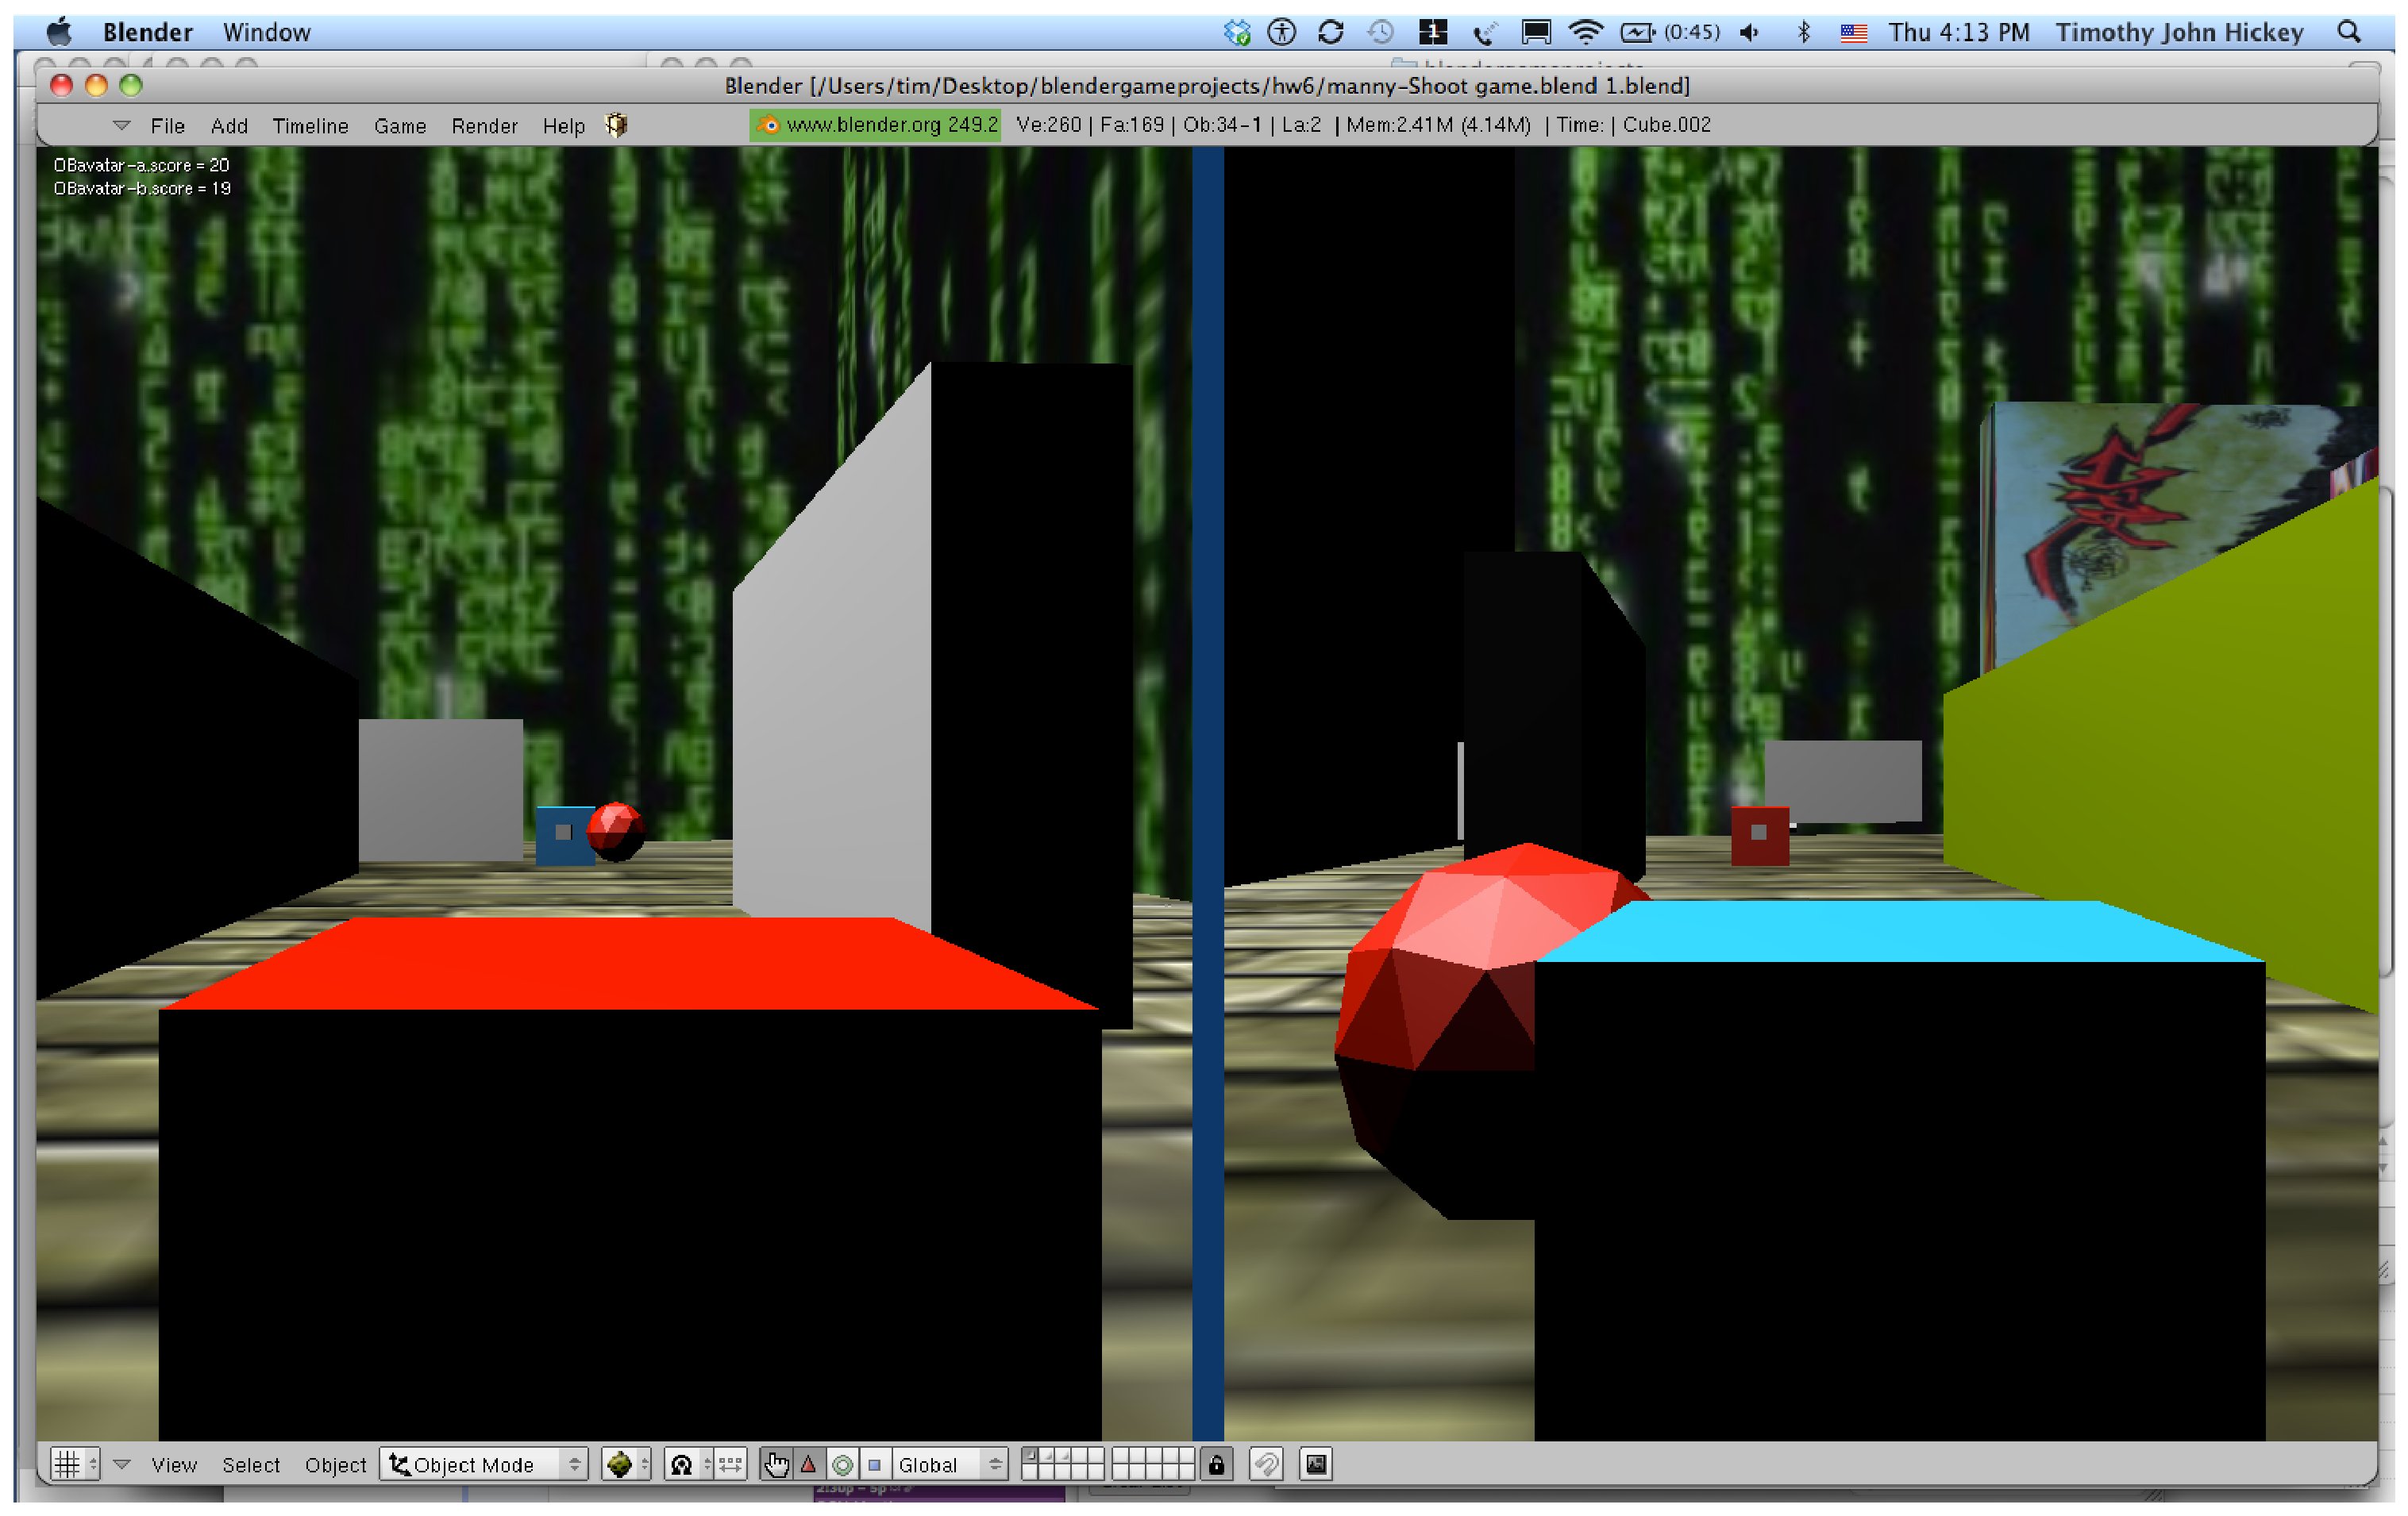
\epsfig{file=shootgame.eps,width=2.5in}
\caption{A split screen shooting game developed in the TYP class}
\label{fig:ssgame}
\end{figure}

\subsubsection{ dominoe games} The games are created by importing or creating simple objects including boxes and sphere, some of which are static and unchanging, others are dynamic and respond to the force of gravity and the impact of other objects. The Physics is computed using the built-in Bullet Physics engine which accounts for rigid body mechanics including friction, gravity, collision elasticity, mass, external forces and torques, and other more sophisticated features such as ball-and-socket joint constraints, hinge constraints, etc. Typically the students create a 3D scene involving a mixture of dominoes and balls on various flat and inclined lanes which create an interesting cascading sequence
of events when the simulation is initiated by hitting the "P" key. In this project the students learn to build structures that interact with the physics engine and develop the basic Blender manipulation skills of
creating, transforming and setting the properties of objects as well as changing views.
\subsubsection{ maze and quest games}
This is a class of game where they learn to create an avatar and associate key press events with actions that apply forces and torques to the avatar. These games involve the user moving an avatar through a
3d world they have constructed using the Sensor/Controller/Actuator logic brick model. They learn how
to change camera views by key presses, switch to different levels (e.g. Win or Lose) when colliding with
the goal object or poison objects, update health points and wealth points. This can all be done using 
the logic bricks and by declaring local health and wealth variables (integer values) for the avatar.


\subsubsection{multi-player (shared keyboard) racing games}
At this point we introduce Python controllers which can be used to create different viewports associated
to different cameras (one for each avatar) or for heads up displays. Students are also introduced to the
general structure of a Python controller which can access the sensors and based on their values,
set the properties of the associated actuators. In the Fall 2010 version of the class we just touched on this part of the Blender application, but in the future we plan to focus a great deal more attention since this is the crucial point at which the transition from visual programming to textual programming is made and where the notions of class, method, module,  variable, constant, expression, and the standard data and control structures are introduced.
\subsubsection{3d simulations of organic chemistry reactions}
The TYP class collaborated with a college-level Honors Organic Chemistry course to create 3d animations of organic reactionss that the chemistry students had researched from current literature. This collaboration resulted in a set of 3d animations of molecular reactions that could potentially be used in future organic chemistry classes. Although the TYP students did learn quite a bit about 3D animation and some organic chemistry, this assignment took us away from the Game Design theme and prevented us from exploring Python controllers in any depth. In the future we will focus only on Game Design and not be distracted by these fascinating but off-topic problem sets.

\subsection{Resources used in class}
\subsubsection{ online tutorials from the Blender community}
The students made extensive use of the online video tutorials created by members of the Blender
community. This was especially true in the first few weeks of the course when they were learning the
basics of the Blender UI and the learning curve is very steep in the beginning since the Blender UI is designed for experts and doesn't yet have a beginner level that has proved so successful with
Dr. Scheme
% include reference here

\subsubsection{screen recordings and student blender project files}
Several lectures were screenrecorded and those recordings were posted to the class website, the
students also learned to create screenrecordings and created tutorials for some of the interesting
parts of their 3D Game Design projects. These tutorials were made available to other students along
with the Blender files showing the final result of the tutorials. These screenrecordings created by
students and for students could be the most powerful type of deliverable generated by this sort of
project. It provides a way for students to contribute to the project in a meaningful way and it also allows
them to learn how to create games by listening to their peers explain it to them. 


\subsubsection{student blogs, sites, docs}
The students commented on some of their assignments and on their peers comments using standard blogging software. They were also required to create and use google sites and googe docs to collaborate in their group projects with other TYP students and with the organic Chemistry students.

\subsection{Evaluation of the TYP 3DGD class}
The initial pilot trial of the TYP 3D Game Design was a qualified success. 

It validated our
assumption that 3D Game Design would be a powerful motivator, at least for some of the students.
There were several groups that invested substantial amounts of time developing their games and this included independent web research to find and learn to use techniques that had not been taught in
class (e.g. throwing objects from the avatar).  The version of blender we used (2.49a) has a notoriously
complex User Interface and this generated quite a bit of frustration among many students. The latest
version of Blender (2.59 stable) features a completely redesigned User Interface and we expect many
fewer problems. It also provides the ability to customize the interface using Python so that one could,
in principle, create different language levels with custom panels showing only the features needed for the 
initial programming projects.

It also demonstrated that the 20material is accessible to students with no prior programming background, all 20 students (10 male/ 10 female) were able complete all of the programming projects
and create fairly interesting and playable 3D games.  Their final projects could all have been improved,
and would have been better if we had not taken a 4 week diversion to collaborate with the Organic Chemistry class to created 3D animations of chemical reactions.  In the future we will try that collaboration with an upper level 3d animation course, but not in this intro level course. The submitted final projects all had realistic skyboxes, interesting sound tracks, appropriate sound effects, challenging game play, and a lot of individual character demonstrating the high level of creativity that went in to creating them. They were also all split screen two player games and the students created these games from scratch using the visual programming logic brick feature to implement all functionality. 

About a third of the students have indicated an interest in continuing in Computer Science and five went on to take another intro course (teaching HTML, Scratch, and Javascript) and three of the students presented their projects in the New England Undergraduate Computing Symposium in the Spring semester and generated quite a bit of interest and excitement among the other undergraduates attending the event.
 

\section{Future Plans: Scaling up}
After this successful pilot study we feel confident in recommending this approach to other educators that are interested in using 3D Game Design to tackle the ethnic/racial diversity problem in Computer Science. We will be offering a revised version of the TYP course during Fall 2011 and will simultaneously focus on developing teaching and learning resources that can be used by other students and educators. The grand challenge however is to find an approach that can scale up to effect the lives of millions of students.  We will begin to explore several different approaches to this scaling problem as described below:


\subsection{After School Courses for High School students}
We have started to collaborate with several local high schools who are interested in having us offer
an after school class in 3D Game Design for their students.  Such a class would help us address the opportunity cost issues and determine whether 3d Game Design is perceived to be a better use of a high school students time than after-school sports, after-school part-time jobs, and other demands on students time.

\subsection{Community Center Workshops}
Several community centers have also expressed interest in having us teach a 3D Game Design course
targeted to high school students. This is an attractive option as such community centers are already
gathering places for many students and they have the expertise to market and run such courses.

\subsection{Citizen Schools}
We have not yet tried to teach 3D Game Design in blender to Middle School students, but 
Citizen Schools has a strong track record of offering interesting and academically challenging
courses to middle school students in at risk districts.

\subsection{Using 3DGD as a core for the new AP course}
A more ambitious approach would be to use 3D Game Design in Blender or another tool as the
core computational paradigm in a new CS AP course. There is currently an effort to create a new
AP course based on Computational Thinking and a Blender-based course would fit will into that
project.

\subsection{3D Game Design Festivals - build it and they will come!}
Based on our positive experience with the game design projects exhibited at the 
New England Undergraduate Computing Symposium, we are planning on organizing a
3D Game Design Festival with competitions for students at different levels (high school, college,
middle school) and using different technology (blender, unity, other). It is easy to run these
festivals online, but more exciting to have a real-life festival.


\subsection{Commons-based Collaborative Mega-courses}
One of the most exciting opportunities to scale up this type of project is to adopt the
Stanford University  "pubic course" approach in which they allow the general public to
enroll in their course and they use web-based tools to provide support and evaluation
of progress. The three courses currently offered at Stanford this semester have well over
200,000 students from the general public that have enrolled.  This approach seems to be
a natural fit for the 3D Game Design project and if successful would provide a powerful
tool for giving students in under-resourced schools access to an education in fundamental
Computer Science concepts.


\section{Conclusions}
The lack of racial/ethnic diversity in Computer Science at all levels is a critical problem of national
concern and it is one that Computer Science educators are well-positioned to address. This paper
has presented one approach to tackling this problem and has described our initial pilot project and
current plans for the next steps.

%ACKNOWLEDGMENTS are optional
\section*{Acknowledgments}
We gratefully acknowledge the students and administrators in the Transitional Year Program
for their willingness to explore this new approach to Computer Science pedagogy. We are also
thankful to the Blender foundation and the Blender community for providing the software and
other resources needed to teach 3D modeling, animation, and game design.

%
% The following two commands are all you need in the
% initial runs of your .tex file to
% produce the bibliography for the citations in your paper.
\bibliographystyle{abbrv}
\bibliography{sigproc}  % sigproc.bib is the name of the Bibliography in this case
% You must have a proper ".bib" file
%  and remember to run:
% latex bibtex latex latex
% to resolve all references
%
% ACM needs 'a single self-contained file'!
%

\section*{References}
Generated by bibtex from your ~.bib file.  Run latex,
then bibtex, then latex twice (to resolve references)
to create the ~.bbl file.  Insert that ~.bbl file into
the .tex source file and comment out
the command \texttt{{\char'134}thebibliography}.
% This next section command marks the start of
% Appendix B, and does not continue the present hierarchy

%\balancecolumns % GM June 2007
% That's all folks!
\end{document}
